\documentclass[a4paper,12pt]{article}
\usepackage[margin=18mm]{geometry}
\usepackage{tikz}
\usepackage{amsmath}
\newcommand{\pFourCell}[2]{\makebox[#1em][c]{\ensuremath{#2}}}
\pagestyle{empty}
\begin{document}
\section*{Spaltentreue LaTeX-Ausgabe}
\noindent Gleichung: \texttt{2*sqrt((x+3)/(2+1))=5} \hfill Zielvariable: \texttt{x} \hfill Profil: \texttt{standard}

\vspace{8mm}
\begin{center}
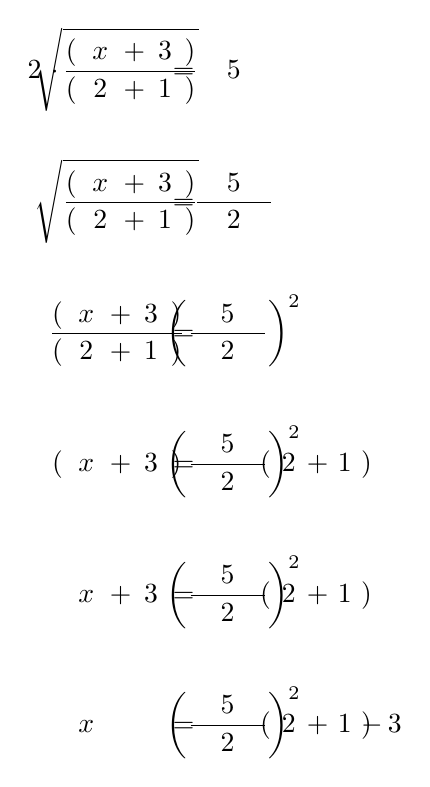
\begin{tikzpicture}[x=1em,y=-1em]
\node[anchor=base, inner sep=0pt] at (0.44,2.9) {$2$};
\node[anchor=base, inner sep=0pt] at (1.17,2.9) {$\cdot$};
\node[anchor=base, inner sep=0pt] at (3.41,2.9) {$\sqrt{\displaystyle\frac{\left(\pFourCell{1.7}{x}\pFourCell{0.78}{+}\pFourCell{1.42}{3}\right)}{\left(\pFourCell{1.7}{2}\pFourCell{0.78}{+}\pFourCell{1.42}{1}\right)}}$};
\node[anchor=base, inner sep=0pt] at (5.83,2.9) {$=$};
\node[anchor=base, inner sep=0pt] at (7.64,2.9) {$5$};
\node[anchor=base, inner sep=0pt] at (7.64,7.65) {$\displaystyle\frac{\pFourCell{2.68}{5}}{\pFourCell{2.68}{2}}$};
\node[anchor=base, inner sep=0pt] at (3.41,7.65) {$\sqrt{\displaystyle\frac{\left(\pFourCell{1.7}{x}\pFourCell{0.78}{+}\pFourCell{1.42}{3}\right)}{\left(\pFourCell{1.7}{2}\pFourCell{0.78}{+}\pFourCell{1.42}{1}\right)}}$};
\node[anchor=base, inner sep=0pt] at (5.83,7.65) {$=$};
\node[anchor=base, inner sep=0pt] at (3.41,12.385) {$\displaystyle\frac{\left(\pFourCell{1.7}{x}\pFourCell{0.78}{+}\pFourCell{1.42}{3}\right)}{\left(\pFourCell{1.7}{2}\pFourCell{0.78}{+}\pFourCell{1.42}{1}\right)}$};
\node[anchor=base, inner sep=0pt] at (5.83,12.385) {$=$};
\node[anchor=base, inner sep=0pt] at (7.64,12.385) {$\left(\displaystyle\frac{\pFourCell{2.68}{5}}{\pFourCell{2.68}{2}}\right)^{2}$};
\node[anchor=base, inner sep=0pt] at (3.41,17.105) {$\left(\pFourCell{1.7}{x}\pFourCell{0.78}{+}\pFourCell{1.42}{3}\right)$};
\node[anchor=base, inner sep=0pt] at (5.83,17.105) {$=$};
\node[anchor=base, inner sep=0pt] at (7.64,17.105) {$\left(\displaystyle\frac{\pFourCell{2.68}{5}}{\pFourCell{2.68}{2}}\right)^{2}$};
\node[anchor=base, inner sep=0pt] at (10.61,17.105) {$\left(\pFourCell{1.3}{2}\pFourCell{0.78}{+}\pFourCell{1.18}{1}\right)$};
\node[anchor=base, inner sep=0pt] at (2.31,21.825) {$x$};
\node[anchor=base, inner sep=0pt] at (3.55,21.825) {$+$};
\node[anchor=base, inner sep=0pt] at (4.65,21.825) {$3$};
\node[anchor=base, inner sep=0pt] at (5.83,21.825) {$=$};
\node[anchor=base, inner sep=0pt] at (7.64,21.825) {$\left(\displaystyle\frac{\pFourCell{2.68}{5}}{\pFourCell{2.68}{2}}\right)^{2}$};
\node[anchor=base, inner sep=0pt] at (10.61,21.825) {$\left(\pFourCell{1.3}{2}\pFourCell{0.78}{+}\pFourCell{1.18}{1}\right)$};
\node[anchor=base, inner sep=0pt] at (2.31,26.545) {$x$};
\node[anchor=base, inner sep=0pt] at (5.83,26.545) {$=$};
\node[anchor=base, inner sep=0pt] at (7.64,26.545) {$\left(\displaystyle\frac{\pFourCell{2.68}{5}}{\pFourCell{2.68}{2}}\right)^{2}$};
\node[anchor=base, inner sep=0pt] at (10.61,26.545) {$\left(\pFourCell{1.3}{2}\pFourCell{0.78}{+}\pFourCell{1.18}{1}\right)$};
\node[anchor=base, inner sep=0pt] at (12.63,26.545) {$-$};
\node[anchor=base, inner sep=0pt] at (13.46,26.545) {$3$};
\end{tikzpicture}
\end{center}

\newpage
\section*{Spaltentreue LaTeX-Ausgabe mit Spaltengrenzen}
\vspace{6mm}
\begin{center}
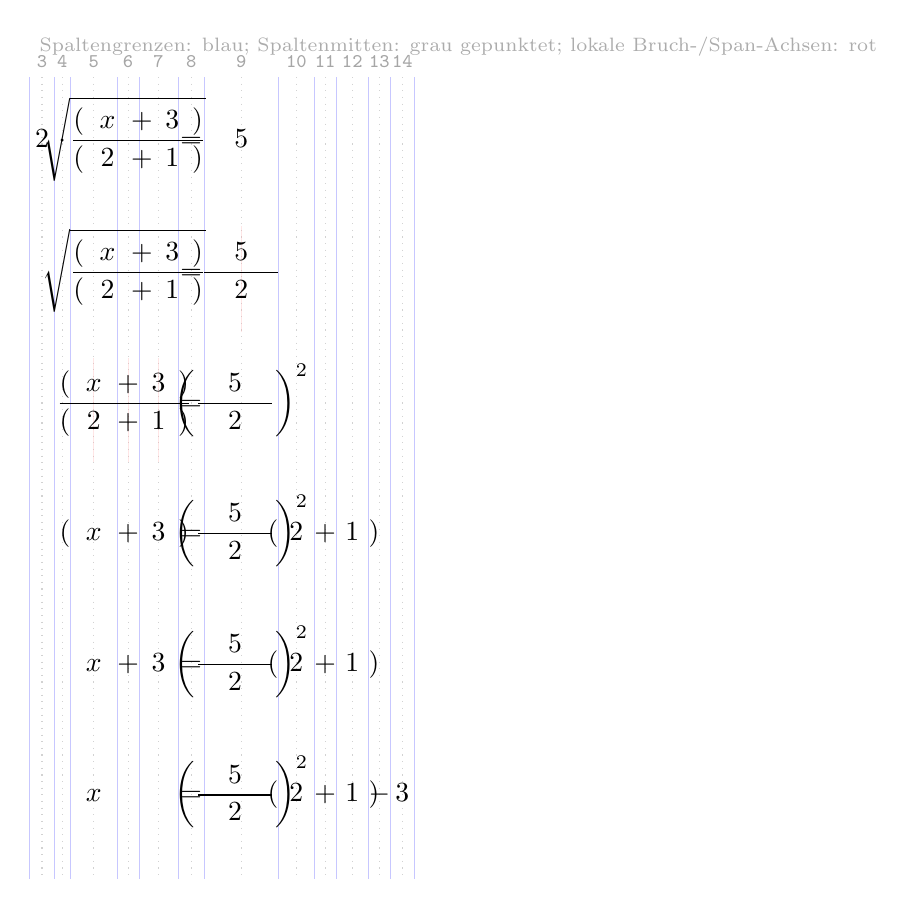
\begin{tikzpicture}[x=1em,y=-1em]
\node[font={\scriptsize}, text=gray!65, anchor=west] at (0,-0.75) {Spaltengrenzen: blau; Spaltenmitten: grau gepunktet; lokale Bruch-/Span-Achsen: rot};
\draw[blue!22, line width=0.28pt] (0,0.35) -- (0,29.33);
\draw[blue!22, line width=0.28pt] (0.88,0.35) -- (0.88,29.33);
\draw[blue!22, line width=0.28pt] (1.46,0.35) -- (1.46,29.33);
\draw[blue!22, line width=0.28pt] (3.16,0.35) -- (3.16,29.33);
\draw[blue!22, line width=0.28pt] (3.94,0.35) -- (3.94,29.33);
\draw[blue!22, line width=0.28pt] (5.36,0.35) -- (5.36,29.33);
\draw[blue!22, line width=0.28pt] (6.3,0.35) -- (6.3,29.33);
\draw[blue!22, line width=0.28pt] (8.98,0.35) -- (8.98,29.33);
\draw[blue!22, line width=0.28pt] (10.28,0.35) -- (10.28,29.33);
\draw[blue!22, line width=0.28pt] (11.06,0.35) -- (11.06,29.33);
\draw[blue!22, line width=0.28pt] (12.24,0.35) -- (12.24,29.33);
\draw[blue!22, line width=0.28pt] (13.02,0.35) -- (13.02,29.33);
\draw[blue!22, line width=0.28pt] (13.9,0.35) -- (13.9,29.33);
\draw[gray!35, dotted] (0.44,0.35) -- (0.44,29.33);
\node[font={\ttfamily\scriptsize}, text=gray!70, anchor=base] at (0.44,0) {3};
\draw[gray!35, dotted] (1.17,0.35) -- (1.17,29.33);
\node[font={\ttfamily\scriptsize}, text=gray!70, anchor=base] at (1.17,0) {4};
\draw[gray!35, dotted] (2.31,0.35) -- (2.31,29.33);
\node[font={\ttfamily\scriptsize}, text=gray!70, anchor=base] at (2.31,0) {5};
\draw[gray!35, dotted] (3.55,0.35) -- (3.55,29.33);
\node[font={\ttfamily\scriptsize}, text=gray!70, anchor=base] at (3.55,0) {6};
\draw[gray!35, dotted] (4.65,0.35) -- (4.65,29.33);
\node[font={\ttfamily\scriptsize}, text=gray!70, anchor=base] at (4.65,0) {7};
\draw[gray!35, dotted] (5.83,0.35) -- (5.83,29.33);
\node[font={\ttfamily\scriptsize}, text=gray!70, anchor=base] at (5.83,0) {8};
\draw[gray!35, dotted] (7.64,0.35) -- (7.64,29.33);
\node[font={\ttfamily\scriptsize}, text=gray!70, anchor=base] at (7.64,0) {9};
\draw[gray!35, dotted] (9.63,0.35) -- (9.63,29.33);
\node[font={\ttfamily\scriptsize}, text=gray!70, anchor=base] at (9.63,0) {10};
\draw[gray!35, dotted] (10.67,0.35) -- (10.67,29.33);
\node[font={\ttfamily\scriptsize}, text=gray!70, anchor=base] at (10.67,0) {11};
\draw[gray!35, dotted] (11.65,0.35) -- (11.65,29.33);
\node[font={\ttfamily\scriptsize}, text=gray!70, anchor=base] at (11.65,0) {12};
\draw[gray!35, dotted] (12.63,0.35) -- (12.63,29.33);
\node[font={\ttfamily\scriptsize}, text=gray!70, anchor=base] at (12.63,0) {13};
\draw[gray!35, dotted] (13.46,0.35) -- (13.46,29.33);
\node[font={\ttfamily\scriptsize}, text=gray!70, anchor=base] at (13.46,0) {14};
\node[anchor=base, inner sep=0pt] at (0.44,2.9) {$2$};
\node[anchor=base, inner sep=0pt] at (1.17,2.9) {$\cdot$};
\node[anchor=base, inner sep=0pt] at (3.41,2.9) {$\sqrt{\displaystyle\frac{\left(\pFourCell{1.7}{x}\pFourCell{0.78}{+}\pFourCell{1.42}{3}\right)}{\left(\pFourCell{1.7}{2}\pFourCell{0.78}{+}\pFourCell{1.42}{1}\right)}}$};
\node[anchor=base, inner sep=0pt] at (5.83,2.9) {$=$};
\node[anchor=base, inner sep=0pt] at (7.64,2.9) {$5$};
\draw[red!30, opacity=0.32, line width=0.35pt] (7.64,5.75) -- (7.64,9.55);
\node[anchor=base, inner sep=0pt] at (7.64,7.65) {$\displaystyle\frac{\pFourCell{2.68}{5}}{\pFourCell{2.68}{2}}$};
\node[anchor=base, inner sep=0pt] at (3.41,7.65) {$\sqrt{\displaystyle\frac{\left(\pFourCell{1.7}{x}\pFourCell{0.78}{+}\pFourCell{1.42}{3}\right)}{\left(\pFourCell{1.7}{2}\pFourCell{0.78}{+}\pFourCell{1.42}{1}\right)}}$};
\node[anchor=base, inner sep=0pt] at (5.83,7.65) {$=$};
\draw[red!30, opacity=0.32, line width=0.35pt] (2.31,10.5) -- (2.31,14.27);
\draw[red!30, opacity=0.32, line width=0.35pt] (3.55,10.5) -- (3.55,14.27);
\draw[red!30, opacity=0.32, line width=0.35pt] (4.65,10.5) -- (4.65,14.27);
\node[anchor=base, inner sep=0pt] at (3.41,12.385) {$\displaystyle\frac{\left(\pFourCell{1.7}{x}\pFourCell{0.78}{+}\pFourCell{1.42}{3}\right)}{\left(\pFourCell{1.7}{2}\pFourCell{0.78}{+}\pFourCell{1.42}{1}\right)}$};
\node[anchor=base, inner sep=0pt] at (5.83,12.385) {$=$};
\node[anchor=base, inner sep=0pt] at (7.64,12.385) {$\left(\displaystyle\frac{\pFourCell{2.68}{5}}{\pFourCell{2.68}{2}}\right)^{2}$};
\node[anchor=base, inner sep=0pt] at (3.41,17.105) {$\left(\pFourCell{1.7}{x}\pFourCell{0.78}{+}\pFourCell{1.42}{3}\right)$};
\node[anchor=base, inner sep=0pt] at (5.83,17.105) {$=$};
\node[anchor=base, inner sep=0pt] at (7.64,17.105) {$\left(\displaystyle\frac{\pFourCell{2.68}{5}}{\pFourCell{2.68}{2}}\right)^{2}$};
\node[anchor=base, inner sep=0pt] at (10.61,17.105) {$\left(\pFourCell{1.3}{2}\pFourCell{0.78}{+}\pFourCell{1.18}{1}\right)$};
\node[anchor=base, inner sep=0pt] at (2.31,21.825) {$x$};
\node[anchor=base, inner sep=0pt] at (3.55,21.825) {$+$};
\node[anchor=base, inner sep=0pt] at (4.65,21.825) {$3$};
\node[anchor=base, inner sep=0pt] at (5.83,21.825) {$=$};
\node[anchor=base, inner sep=0pt] at (7.64,21.825) {$\left(\displaystyle\frac{\pFourCell{2.68}{5}}{\pFourCell{2.68}{2}}\right)^{2}$};
\node[anchor=base, inner sep=0pt] at (10.61,21.825) {$\left(\pFourCell{1.3}{2}\pFourCell{0.78}{+}\pFourCell{1.18}{1}\right)$};
\node[anchor=base, inner sep=0pt] at (2.31,26.545) {$x$};
\node[anchor=base, inner sep=0pt] at (5.83,26.545) {$=$};
\node[anchor=base, inner sep=0pt] at (7.64,26.545) {$\left(\displaystyle\frac{\pFourCell{2.68}{5}}{\pFourCell{2.68}{2}}\right)^{2}$};
\node[anchor=base, inner sep=0pt] at (10.61,26.545) {$\left(\pFourCell{1.3}{2}\pFourCell{0.78}{+}\pFourCell{1.18}{1}\right)$};
\node[anchor=base, inner sep=0pt] at (12.63,26.545) {$-$};
\node[anchor=base, inner sep=0pt] at (13.46,26.545) {$3$};
\end{tikzpicture}
\end{center}
\end{document}
